
\section{Diffraction of Light}

Name \rule{2.0in}{0.1pt}\hfill{}Section \rule{1.0in}{0.1pt}\hfill{}Date
\rule{1.0in}{0.1pt}

\textbf{Objective}

To investigate how the interference and diffraction of light waves
combine to form a distinctive pattern and how that pattern can be
used to measure the size of an object.

\textbf{Introduction}

In this laboratory you will investigate the interference and diffraction
of light produced by a laser beam passing through a set of narrow,
adjacent slits. When light passes through a set of slits, each opening
acts as an independent source of waves that can overlap one another
to produce a distinctive pattern of bright and dark spots on a screen.
The position of the bright spots depends on the separation of the
adjacent slits and the wavelength of the incident light. In addition,
diffraction produced by the individual slits modifies the intensity
of each spot. To perform the following activities you will need:

\begin{itemize}
\item Laser.
\item Phototransistor for measuring light intensity (mounted on rotary motion sensor).
\item Set of narrow slits.
\item {\it DataStudio} 750 Interface.
\item Plumb line.
\end{itemize}
You can measure this interference/diffraction pattern with the setup
shown below. A phototransistor is seated behind the narrow opening on top
of the metal mount. The phototransistor can translate the intensity
of the light falling on it into a voltage signal that can be read
by the computer. In addition, the phototransistor can be moved back and
forth on a rotary motion sensor that measures the position of the 
mount.
These two signals can be combined to
make a graph of the intensity as a function of position.

\vspace{0.3cm}
%{\centering \resizebox*{0.75\textwidth}{!}{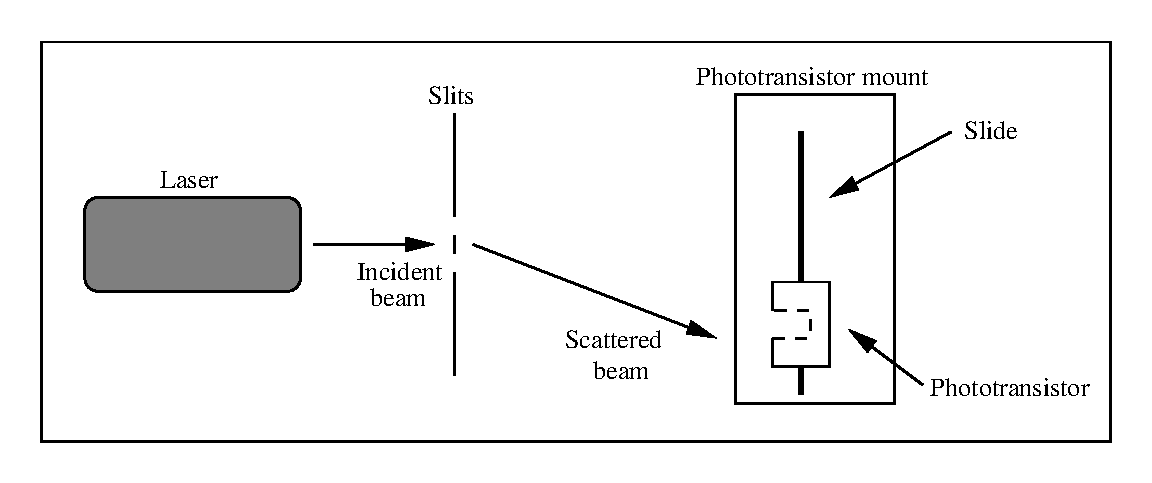
\includegraphics{interference_of_light_fig_1.eps}} \par}
\begin{center}
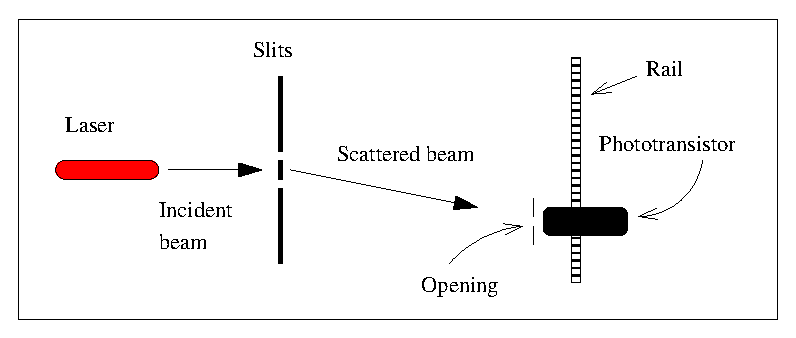
\includegraphics{interference_of_light/interference_of_light_fig1b.eps}
\end{center}
\vspace{0.3cm}

{\centering \textbf{Fig. 1}. View of diffraction apparatus from above.\par}

In this unit you will  pass light of known wavelength through slits 
and use the diffraction pattern to determine the size of the individual
slit through which the light passed.

\textbf{Intensity of Interference }

For light that passes through two very narrow slits one can calculate
a theoretical expression for the interference pattern that would be
produced in such a situation. The expression is 

\begin{displaymath} I_{int} = 4I_0 cos^2 (\frac {\pi d} {\lambda} \sin \theta ) \end{displaymath}

where $I_{int}$ is the intensity of the light at the phototransistor,
$I_{0}$ is the maximum intensity of the incident light, d is
the slit separation, \( \theta  \) is the angular position of the
scattered light relative to the incident beam, and \( \lambda  \)
is the wavelength of the light. This expression has a characteristic
shape shown below. We will compare this prediction of {}``pure''
interference (without diffraction effects) with the measured pattern
in the next activity.

\vspace{0.3cm}
{\centering 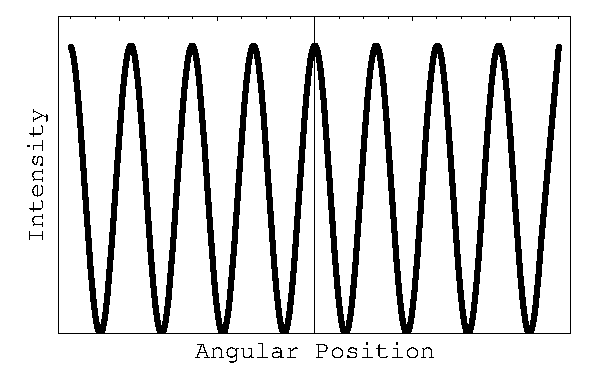
\includegraphics{diffraction_of_light/diffraction_of_light_fig_2.eps} \par}
\vspace{0.3cm}

{\centering \textbf{Fig. 2}. Intensity distribution of pure interference.\par}

\textbf{Activity 1: The Interference of Light }

(a) You are now ready to turn on the laser. DO NOT LOOK DIRECTLY INTO
THE BEAM OR POINT THE LASER CARELESSLY ABOUT THE ROOM. Turn on the
laser and you should see the bright red spot of the beam striking
the wall. You should have a glass plate with a green border and several
different slit arrangements on it. Place the opening in the center
of the plate in the path of the laser beam. The adjacent slits in
the center hole are 0.03295 mm apart.What do you see? 
\vspace{20mm}

(b) Position the glass plate about 30-40 cm from the phototransistor
apparatus with the beam striking the center opening. Place the apparatus
so the intensity pattern is at the same height as the opening in the
center of the device mounted on a movable slide. The phototransistor
is mounted behind this opening. To make accurate measurements it is important
to carefully determine the geometry of your setup. Check to see if
the slits and the phototransistor mount are perpendicular to the incident
laser beam. You also want the phototransistor to {}``see'' as many
bright spots as possible. Gently slide the mount back and forth to
make sure the phototransistor stays centered on the interference pattern.
You need to know the perpendicular distance from the center hole to
the position of the phototransistor. Place the phototransistor mount
at the position of the central maximum (the brightest spot) and measure
the distance from the center hole of the slits to the front face of
the phototransistor mount. You may find it useful to use the plumb
line to measure this distance. Record your result. The phototransistor
itself sits 25.4 mm behind the opening on the front face of the phototransistor
mount.
\vspace{20mm}

(c) Start the ``Interference'' activity in the {\bf 132 Workshop} folder. 
When you are ready, click {\bf Start} and slowly move the phototransistor from one side of the slide to the other by turning the wheel on the rotary motion sensor. Move carefully and take about 4-5 seconds to complete the motion. When data acquisition is complete, click {\bf Stop} and you will see a graph
representing the intensity reading versus the position reading. You
should see several distinct peaks. This graph is the interference
pattern. If you do not see this pattern, consult your instructor.
Make a hardcopy of this graph and attach it to this unit.

(d) Is the spacing between the intensity peaks constant? Is the intensity
of each peak the same? Does it appear that any peaks are missing?
How does the measured intensity spectrum compare with the one predicted
for {}``pure'' interference discussed above? What is different?
What is the same?
\vspace{30mm}

(e) Measure and record the Position Reading and Intensity Reading
of each peak in the table below.
Use the
{\bf Smart Tool} to accurately read off the peak positions by clicking on the
appropriate button along the top of the graph. A set of cross-hairs will appear on the
plot. Grab the cross-hairs by clicking on them and dragging them to the point you want
to measure.
The coordinates will be printed by the cross-hairs.
Turn off the laser when you are finished.

\vspace{0.3cm}
{\centering \begin{tabular}{|c|c|}
\hline 
Position Reading (m)&
Intensity Reading (\%)\\
\hline
\hline 
&
\\
\hline 
&
\\
\hline 
&
\\
\hline 
&
\\
\hline 
&
\\
\hline 
&
\\
\hline 
&
\\
\hline 
&
\\
\hline 
&
\\
\hline
\end{tabular}\par}
\vspace{0.3cm}

\textbf{Activity 2: Intensity of Diffraction} 

Applying the same theoretical techniques that were applied to interference
(see equation above) one can derive a prediction for the intensity
pattern due to diffraction of light passing through a single slit.
The result is 

\begin{displaymath} I_{diff} = I_m (\frac {\sin (\frac {\pi a} {\lambda} \sin \theta)} {\frac {\pi a} {\lambda} \sin \theta} )^2 \end{displaymath}

where $a$ is the size of the single slit, \( \theta  \) is the angular
position of the phototransistor relative to the incident beam, $I_{m}$
is the maximum intensity at the center of the diffraction pattern,
and \( \lambda  \) is the wavelength of the light. The shape of this
intensity distribution is shown in Figure 3.

\vspace{0.3cm}
{\centering 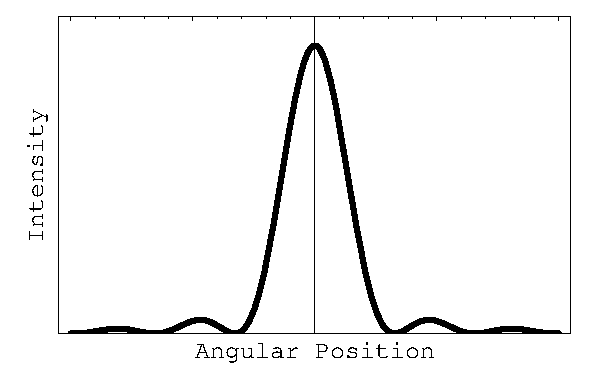
\includegraphics{diffraction_of_light/diffraction_of_light_fig_3.eps} \par}
\vspace{0.3cm}

{\centering \textbf{Fig. 3}. Intensity distribution of diffraction
from a single slit.\par}

(a) The figure above shows the diffraction pattern has a central maximum
with a series of points where the intensity goes to zero at positive
and negative angles. When is the expression for the intensity in the
equation above equal to zero?
\vspace{20mm}

(b) Using the result of part (a), what is the angular position of
the minima on either side of the central maximum?
\vspace{20mm}

(c) Finally, generate an expression for the angular width of the central
maximum in terms of $a$, \( \lambda  \), and any other constants you
need.
\vspace{30mm}

\textbf{Combining Interference and Diffraction}

By now you should have realized that your measured intensity distribution
does not completely agree with the distribution predicted by {}``pure''
interference as represented by the first equation and Figure 2. When
light passes through a pair of slits diffraction occurs at each individual
slit and casts the characteristic pattern described by the second
equation. At the same time there is interference between the light
from different slits that creates an interference pattern described
by the first equation. The net effect is a multiplication of these
two equations to yield 

\begin{displaymath} I_{total} = I_m \cos^2 (\frac {\pi d} {\lambda} \sin \theta ) (\frac {\sin (\frac {\pi a} {\lambda} \sin \theta)} {\frac {\pi a} {\lambda} \sin \theta} )^2 \end{displaymath}

where $I_{m}$ is the intensity of the central maximum, \( \theta  \)
is the position of the phototransistor, $d$ is the separation of the
slits, $a$ is the size of an individual slit, and \( \lambda  \) is
the wavelength of the light. The shape of this distribution is shown
by the solid curve in Figure 4.

\vspace{0.3cm}
{\centering 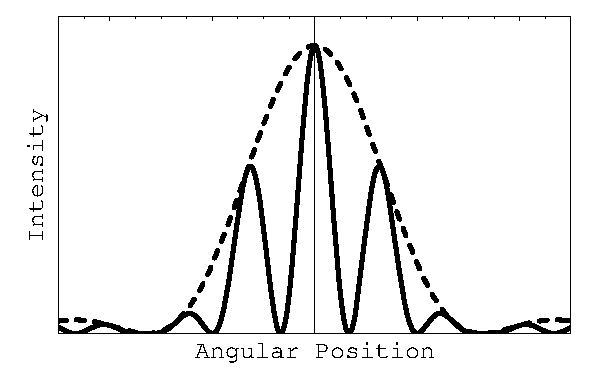
\includegraphics{diffraction_of_light/diffraction_of_light_fig_4.eps} \par}
\vspace{0.3cm}

{\centering \textbf{Fig. 4}. Intensity distribution of light passing
through a pair of slits.\par}

The intensity of the interference peaks is no longer constant, but
is modulated by the diffraction envelope represented by the dashed
curve. This dashed curve is a plot of the second equation normalized
to the maximum intensity at zero degrees. The intensity of each peak
in the distribution represents the intensity due to the diffraction
effects. If more slits are added, then the widths of the individual
peaks in Figure 4 become narrower, but their intensity remains the
same. In the next Activity you will use your data to determine the
diffraction pattern and the angular width of the central diffraction
envelope. This width can be used to measure the size of the individual
slits that produced the distribution.

\textbf{Activity 3: Measuring the Size of the Slit with the Diffraction
Pattern }

(a) Does the intensity distribution you measured with the phototransistor
resemble the pattern shown in Figure 4? If not, consult your instructor.
\vspace{10mm}

(b) In Activity 1 you recorded the position and intensity of the interference
peaks you measured with the phototransistor. How would you calculate
the angular position of each peak relative to the central maximum?
A sketch might be helpful here.
\vspace{30mm}

(c) Use your expression to calculate the angular position of each
interference peak that you recorded and enter your results in the
table below. Plot intensity versus angular position.
Does your plot resemble the shape of the diffraction pattern shown
in Figure 3? If not, consult your instructor. Print the plot and attach
it to this unit.

\vspace{0.3cm}
{\centering \begin{tabular}{|c|c|}
\hline 
Angular Position (radians)&
Intensity Reading (V)\\
\hline
\hline 
&
\\
\hline 
&
\\
\hline 
&
\\
\hline 
&
\\
\hline 
&
\\
\hline 
&
\\
\hline 
&
\\
\hline 
&
\\
\hline 
&
\\
\hline
\end{tabular}\par}
\vspace{0.3cm}

(d) What is the angular width of the central maximum in your data?
Use the expression from part 2(c) to calculate the size of the slit.
The expected result is 0.015 mm. What is your percent difference?
Use the wavelength for the laser light that you found in the unit
on interference of light.
\vspace{30mm}

(e) Collect the results for the slit width from the other teams in class
and calculate the average and standard deviation. Record the result here.
Are your results consistent with the class results? Why or why not?
\vspace{60mm}

(f) Can you think of any other methods for measuring small separations
like this accurately?
